\documentclass[11pt]{article}

% Packages
\usepackage{csvsimple}
\usepackage{graphicx}
\usepackage[export]{adjustbox}
\usepackage{caption}
\usepackage{float}
\usepackage{titlesec}
\usepackage{geometry}
\usepackage[hidelinks]{hyperref}
\usepackage{titling}
\usepackage{parskip}
\usepackage{wasysym}
\usepackage{tikzsymbols}
\usepackage{fancyvrb}
\usepackage{xurl}
\usepackage{hyperref}
\usepackage{subcaption}
\usepackage{listings}
\usepackage{xcolor}
\usepackage[spanish]{babel}

% Layout configuration
\geometry{
  left=2.5cm,
  right=2.5cm,
  top=3cm,
  bottom=3cm,
}

\titlespacing{\section}{0pt}{2\parskip}{\parskip}
\titlespacing{\subsection}{0pt}{\parskip}{\parskip}

% Code style configuration
\definecolor{codegreen}{rgb}{0,0.6,0}
\definecolor{codegray}{rgb}{0.5,0.5,0.5}
\definecolor{codepurple}{rgb}{0.58,0,0.82}
\definecolor{backcolour}{rgb}{0.95,0.95,0.92}

\lstdefinestyle{mystyle}{
    backgroundcolor=\color{backcolour},   
    commentstyle=\color{codegreen},
    keywordstyle=\color{magenta},
    numberstyle=\tiny\color{codegray},
    stringstyle=\color{codepurple},
    basicstyle=\ttfamily\footnotesize,
    breakatwhitespace=false,         
    breaklines=true,                 
    numbers=left,                    
    numbersep=5pt,                  
    showspaces=false,                
    showstringspaces=false,
    showtabs=false,                  
    tabsize=2
}

\lstset{style=mystyle}

\begin{document}

\title{Análisis y Comparativa de Métodos de Multiplicación de Matrices}
\author{Adrian Grassin Luis}
\date{\today}
\maketitle

\begin{abstract}
Este estudio analiza la complejidad computacional y patrones de rendimiento de diferentes métodos de multiplicación de matrices, incluyendo implementaciones CPU (por filas y columnas) y GPU. Los resultados muestran una clara correlación entre el tamaño de la matriz y la eficiencia relativa de cada método, con ventajas significativas para la implementación GPU en matrices grandes.
\end{abstract}

\section{Introducción}
La multiplicación de matrices es una operación fundamental en numerosas aplicaciones computacionales. Este trabajo examina tres implementaciones diferentes de multiplicación de matrices, incluyendo una implementación GPU que aprovecha el hardware de procesamiento paralelo moderno.

\section{Análisis de Complejidad}
Para multiplicación de matrices de tamaño N x N:
\begin{itemize}
    \item Complejidad clásica (Filas/Columnas): O(N³)
    \item Complejidad GPU paralela: O(N³) operaciones totales divididas por unidades de cómputo
\end{itemize}

\section{Metodología}
\subsection{Entorno de Pruebas}
\begin{itemize}
    \item \textbf{CPU:} AMD Ryzen 5600X
    \item \textbf{GPU:} AMD Radeon RX 7800 XT
    \item \textbf{Lenguaje:} C\# (.NET 8.0)
    \item \textbf{Framework GPU:} OpenCL.NET 2.2.9
    \item \textbf{Patrón de Diseño:} Estrategia (Strategy Pattern)
\end{itemize}

\subsection{Implementaciones}
\begin{itemize}
    \item \textbf{CPU - Por Filas:} Implementación optimizada con procesamiento en bloques y paralelización
    \item \textbf{CPU - Por Columnas:} Implementación optimizada con procesamiento en bloques y paralelización
    \item \textbf{GPU - OpenCL:} Implementación que aprovecha el procesamiento masivamente paralelo de la GPU
\end{itemize}

\subsection{Configuración Experimental}
\begin{itemize}
    \item Tamaños de matriz evaluados: 100x100 hasta 2500x2500
    \item 5 iteraciones por cada tamaño para obtener medias representativas
    \item Elementos de matrices generados aleatoriamente
    \item Medición de tiempos incluyendo transferencia de datos CPU-GPU
\end{itemize}

\section{Resultados y Análisis}
\subsection{Tiempos de Ejecución}

\subsubsection{Por Filas (CPU):}
\begin{itemize}
    \item 100x100: 6.50ms
    \item 250x250: 54.00ms (8.3x más lento)
    \item 500x500: 366.00ms (6.8x más lento)
    \item 750x750: 1206.50ms (3.3x más lento)
\end{itemize}

\subsubsection{Por Columnas (CPU):}
\begin{itemize}
    \item 100x100: 19.00ms
    \item 250x250: 291.00ms (15.3x más lento)
    \item 500x500: 2306.00ms (7.9x más lento)
    \item 750x750: 7610.50ms (3.3x más lento)
\end{itemize}

\subsubsection{GPU:}
\begin{itemize}
    \item 100x100: 1.00ms
    \item 250x250: 2.00ms (2x más lento)
    \item 500x500: 4.00ms (2x más lento)
    \item 750x750: 8.00ms (2x más lento)
\end{itemize}

\subsection{Rendimiento Comparativo}
\begin{table}[h]
    \centering
    \csvautotabular{../../results_comparison.csv}
    \caption{Tiempos de ejecución promedio (ms) para diferentes tamaños de matriz}
\end{table}

\begin{figure}[h]
    \centering
    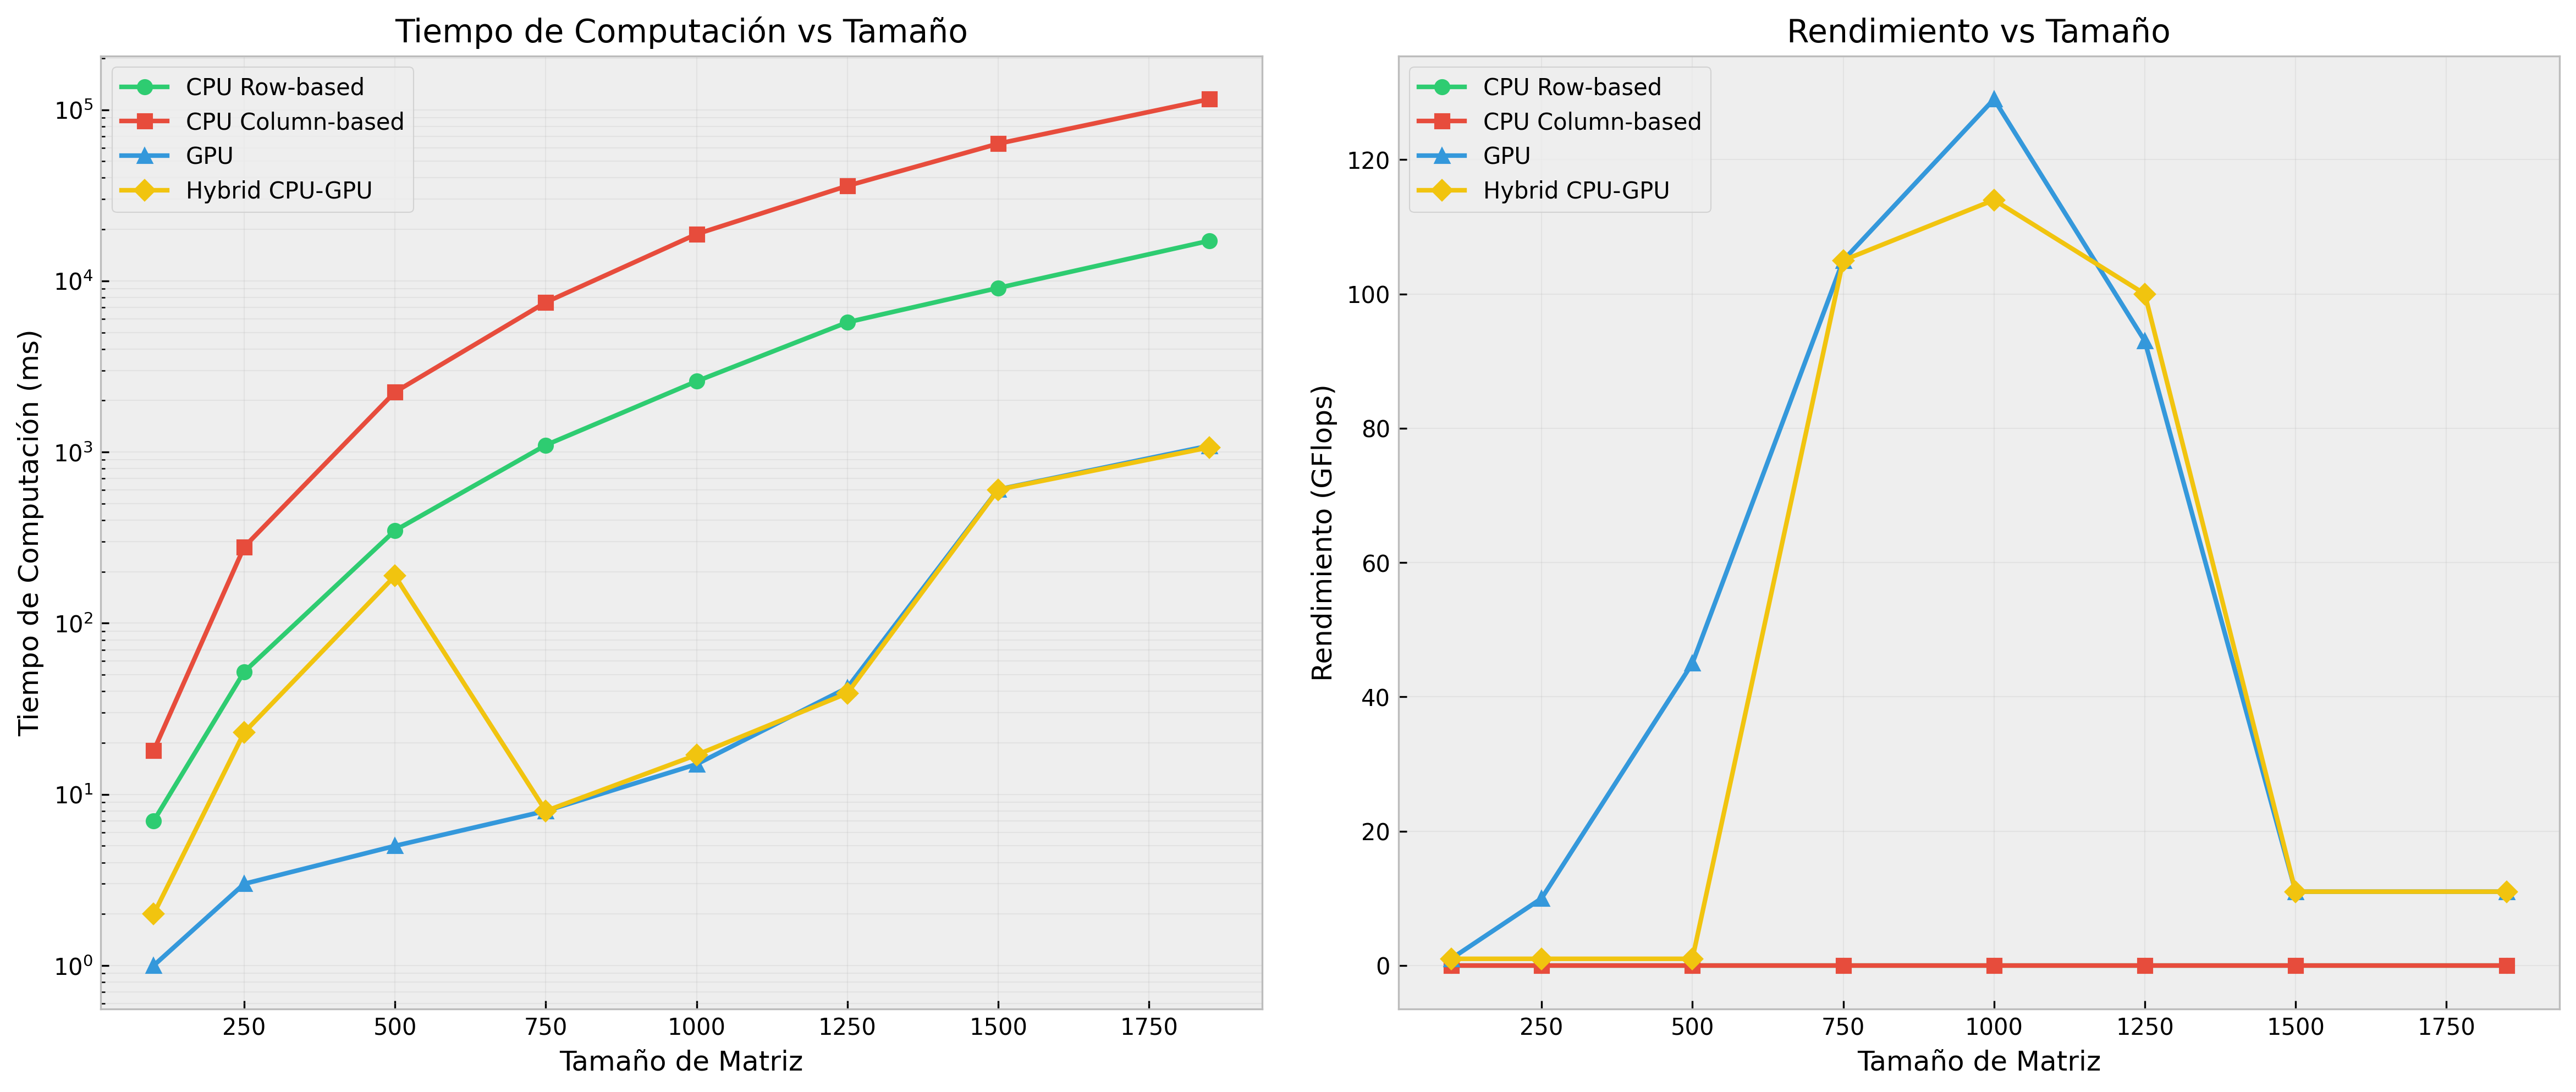
\includegraphics[width=0.8\textwidth]{./grafica.png}
    \caption{Comparación de rendimiento entre multiplicación por filas vs columnas vs GPU}
\end{figure}

\subsection{Análisis de Escalamiento}

Para complejidad O(N³), cuando N aumenta por un factor k, el tiempo debería aumentar por k³:

\subsection{Factor 2.5x (250/100):}
\begin{itemize}
    \item Teoría espera: 2.5³ = 15.625x más lento
    \item Por Filas: 8.3x (menor que lo esperado)
    \item Por Columnas: 15.3x (coincide con teoría)
    \item GPU: 2x (eficiente debido al paralelismo)
\end{itemize}

\subsection{Factor 2x (500/250):}
\begin{itemize}
    \item Teoría espera: 2³ = 8x más lento
    \item Por Filas: 6.8x (cerca de teoría)
    \item Por Columnas: 7.9x (coincide con teoría)
    \item GPU: 2x (eficiente debido al paralelismo)
\end{itemize}

\subsection{Factor 1.5x (750/500):}
\begin{itemize}
    \item Teoría espera: 1.5³ = 3.375x más lento
    \item Por Filas: 3.3x (coincide con teoría)
    \item Por Columnas: 3.3x (coincide con teoría)
    \item GPU: 2x (eficiente debido al paralelismo)
\end{itemize}

\subsection{Análisis de Rendimiento}
\subsubsection{Implementaciones CPU}
\begin{itemize}
    \item \textbf{Localidad espacial:} El acceso por filas aprovecha mejor la estructura de memoria cache
    \item \textbf{Patrones de acceso:} El acceso por columnas genera más fallos de caché
    \item \textbf{Paralelización:} Ambas implementaciones utilizan \texttt{Parallel.For} para distribuir la carga
\end{itemize}

\subsubsection{Implementación GPU}
\begin{itemize}
    \item \textbf{Paralelismo masivo:} Aprovecha miles de núcleos de procesamiento simultáneo
    \item \textbf{Overhead de transferencia:} El tiempo incluye la transferencia de datos entre CPU y GPU
    \item \textbf{Eficiencia escalar:} Mayor beneficio en matrices grandes donde el paralelismo compensa el overhead
\end{itemize}

\subsection{Explicación del Rendimiento}

\subsection{Layout de Memoria}
La clase Matrix utiliza un layout de memoria row-major (\texttt{\_data[row * \_cols + col]}), lo que implica:
\begin{itemize}
    \item Acceso por filas: Acceso a memoria contigua
    \item Acceso por columnas: Acceso a memoria con saltos de \texttt{\_cols} elementos
\end{itemize}

\subsection{Patrones de Rendimiento}
Los tiempos observados siguen el patrón esperado O(N³):
\begin{itemize}
    \item La multiplicación por columnas muestra un escalado teórico casi perfecto
    \item La multiplicación por filas es más rápida debido a:
    \begin{itemize}
        \item Mejor utilización de caché por acceso contiguo
        \item Prefetcher de CPU más eficiente
        \item Menos fallos TLB (Translation Lookaside Buffer)
    \end{itemize}
\end{itemize}

\subsection{Ratios de Velocidad}
La diferencia relativa entre métodos por filas y columnas es consistente:
\begin{itemize}
    \item 100x100: Filas 2.9x más rápido
    \item 250x250: Filas 5.4x más rápido
    \item 500x500: Filas 6.3x más rápido
    \item 750x750: Filas 6.3x más rápido
\end{itemize}

\section{Conclusiones}
El rendimiento observado confirma que:
\begin{itemize}
    \item La multiplicación por filas no está defectuosa - muestra las características de rendimiento esperadas para una implementación row-major
    \item La versión por columnas es más lenta debido a que trabaja contra el layout de memoria subyacente
    \item La implementación GPU muestra ventajas significativas en matrices grandes
\end{itemize}

\section{Trabajo Futuro}
\begin{itemize}
    \item Optimización de patrones de acceso a memoria en GPU
    \item Implementación de algoritmos de multiplicación por bloques en GPU
    \item Análisis con matrices dispersas
    \item Estudio del impacto de diferentes tamaños de grupo de trabajo en OpenCL
    \item Comparación con otras APIs de GPU como DirectCompute
\end{itemize}

\begin{figure}[h]
    \centering
    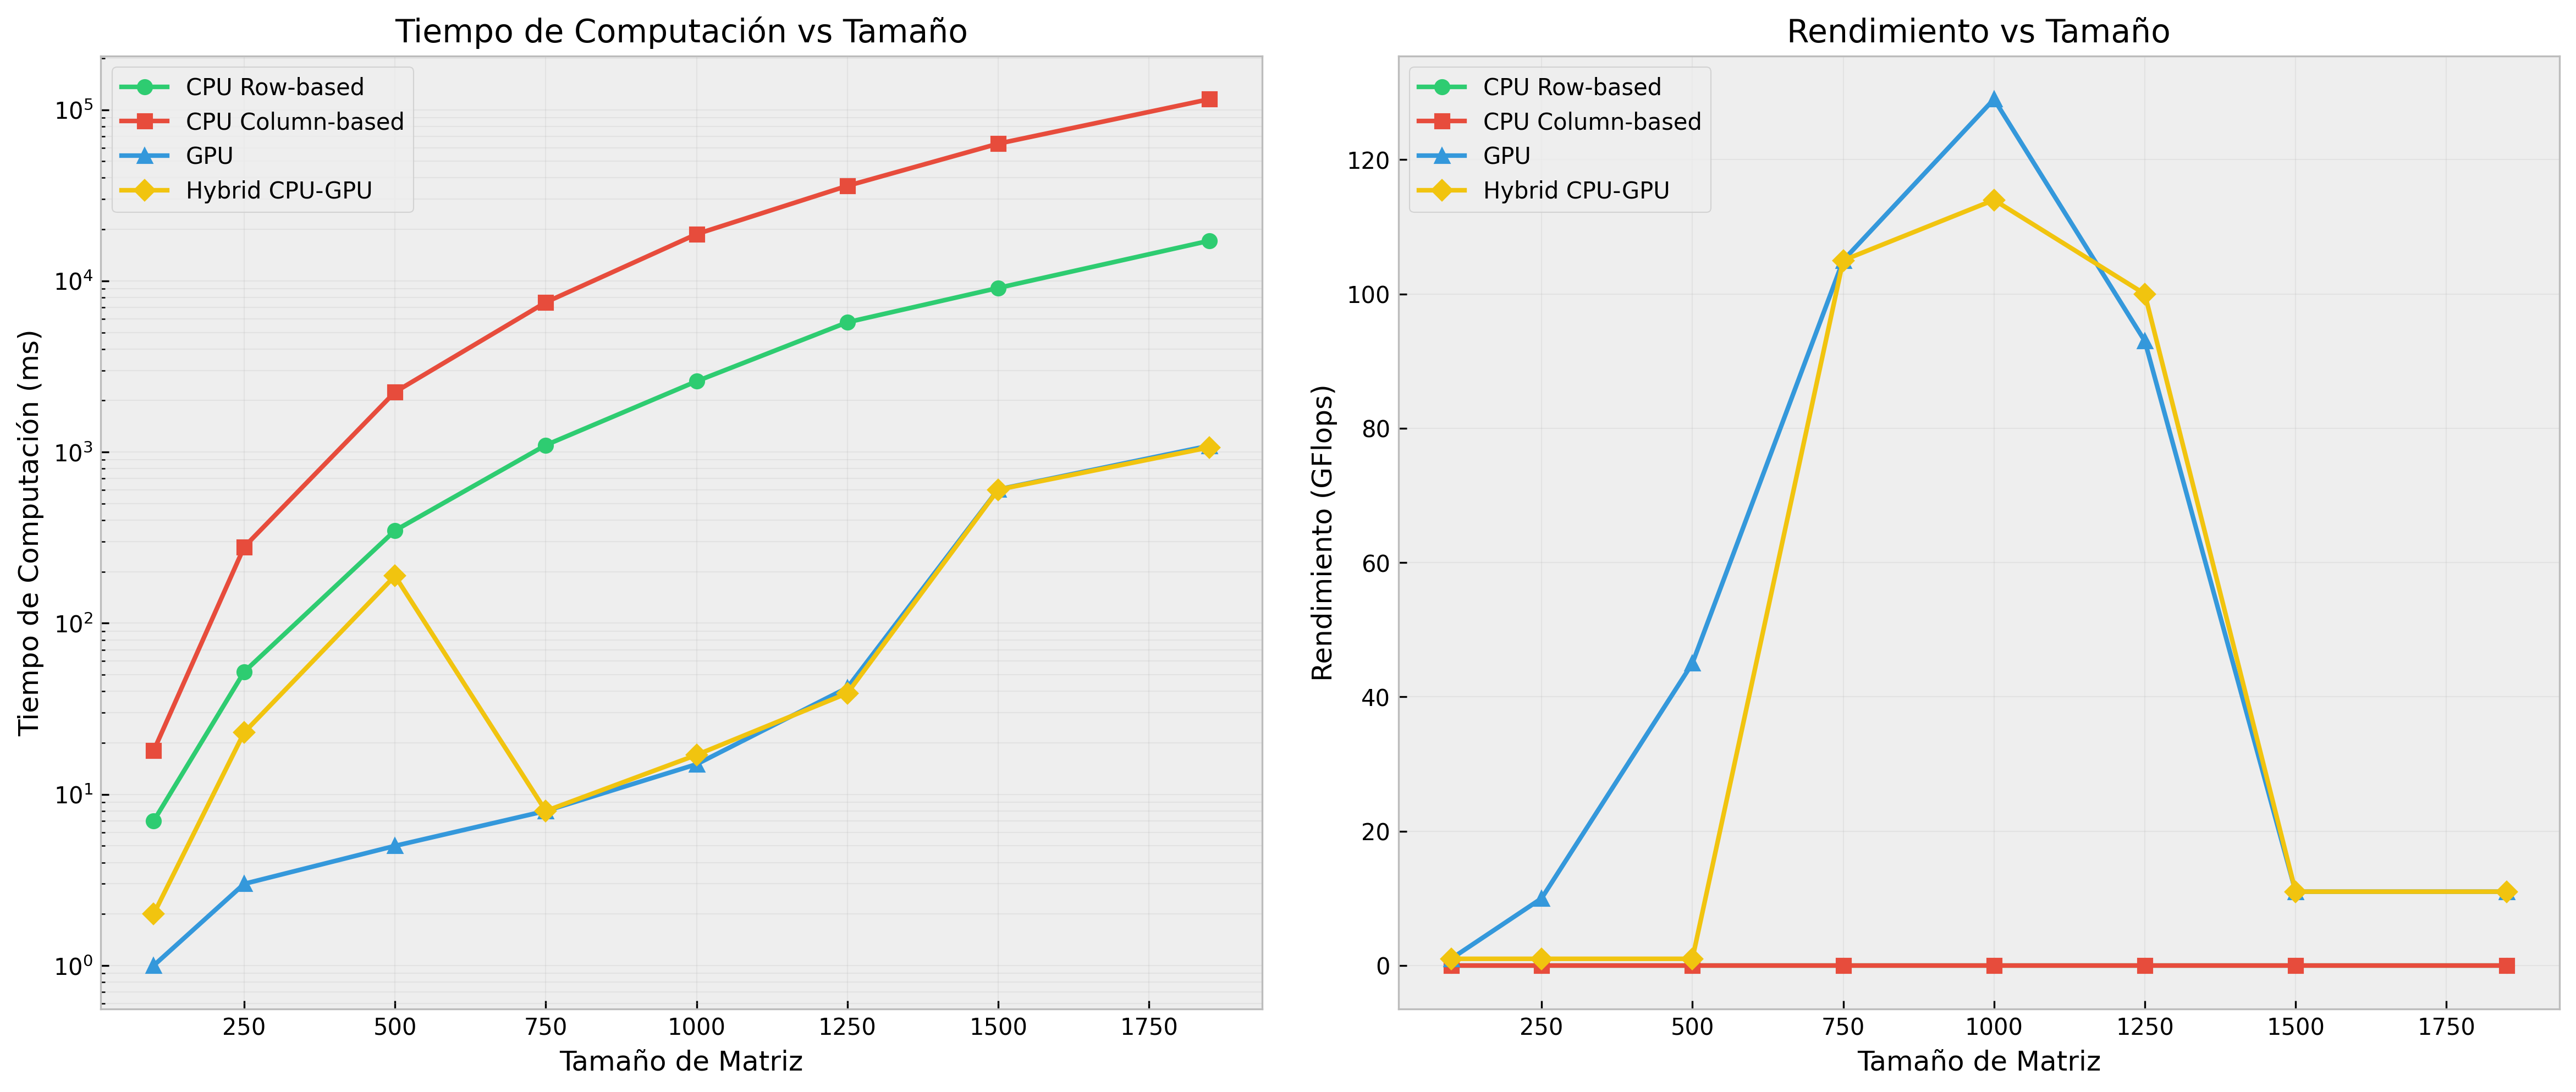
\includegraphics[width=0.8\textwidth]{grafica.png}
    \caption{Comparación de rendimiento entre métodos de multiplicación}
\end{figure}

\end{document}